\chapter{Diseño}
\label{chap:design}

\section{Diseño de la interfaz gráfica}

\subsection{Pantalla de inicio de sesión}

En esta sección se muestra el boceto de la interfaz gráfica del inicio de sesión. Se corresponde con el requisito RF1. 

\begin{figure}[ht]
	\centering
	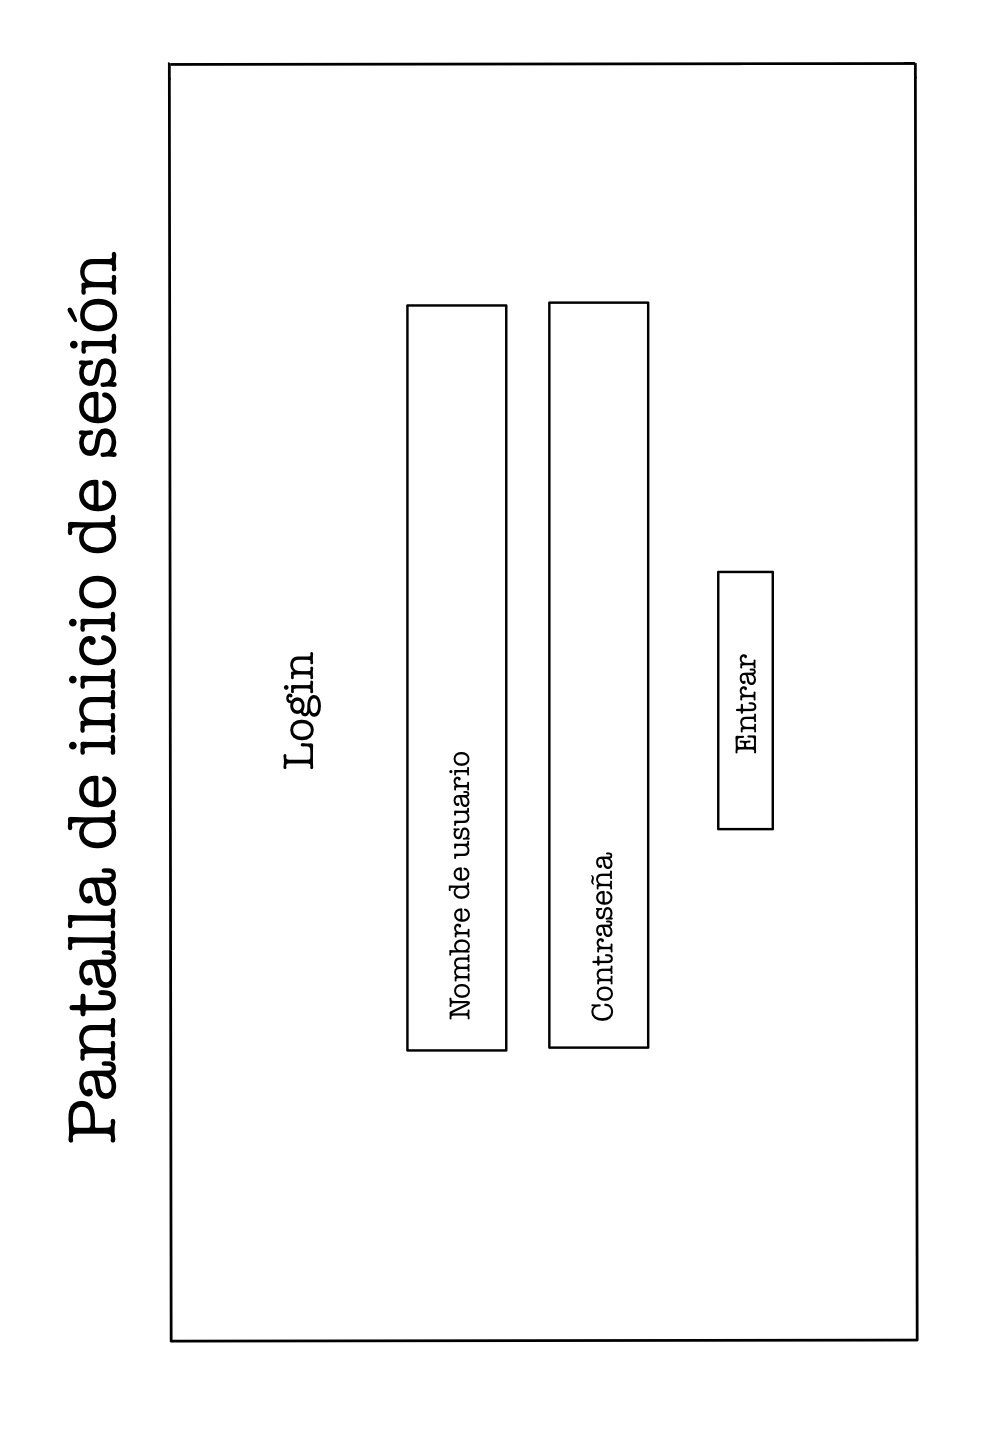
\includegraphics[width=0.7\textwidth, angle=270]{imagenes/inicio_sesion.JPG}
	\caption{Diseño de la pantalla de inicio de sesión.}
	\label{fig:iniciosesion}
\end{figure}


\subsection{Pantalla principal}

En esta sección se muestran los bocetos de la interfaz gráfica de la pantalla principal y las pantallas correspondientes con una nueva venta y un nuevo préstamo. Estas tres pantallas representan los requisitos RF19, RF20 y RF28. Por tanto, es la pantalla que muestra la caja diaria y permite registrar una nueva venta o un nuevo préstamo. 

\begin{figure}[ht]
	\centering
	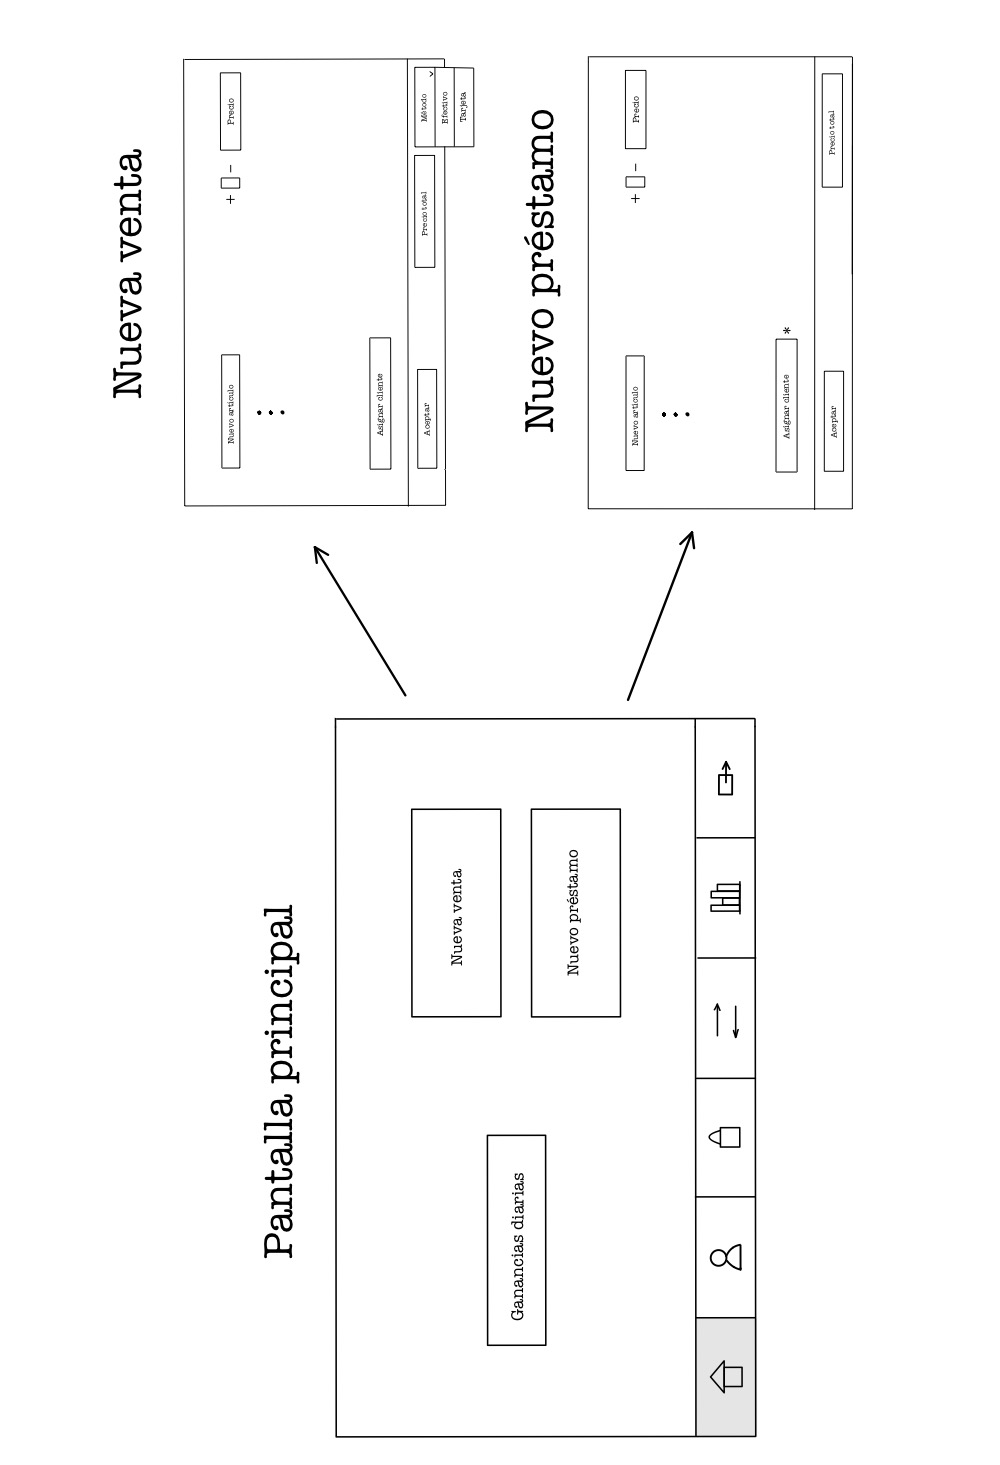
\includegraphics[width=0.8\textwidth, angle=270]{imagenes/pantalla_principal.JPG}
	\caption{Diseño de la pantalla principal.}
	\label{fig:pantallaprincipal}
\end{figure}

\newpage

\subsection{Pantalla de clientes}

En esta sección se muestran los bocetos de la interfaz gráfica de la pantalla clientes. Estas cuatro pantallas representan los requisitos RF12, RF13, RF14, RF15, RF16, RF17 y RF18. En la pantalla clientes podemos ver la lista de clientes existentes, buscar clientes por nombre y filtrar aquellos clientes que tengan préstamos. Si pulsamos encima del nombre del cliente, visualizaremos todos los datos relacionados con este. Además, podemos editar, eliminar y añadir un nuevo cliente. 


\begin{figure}[ht]
	\centering
	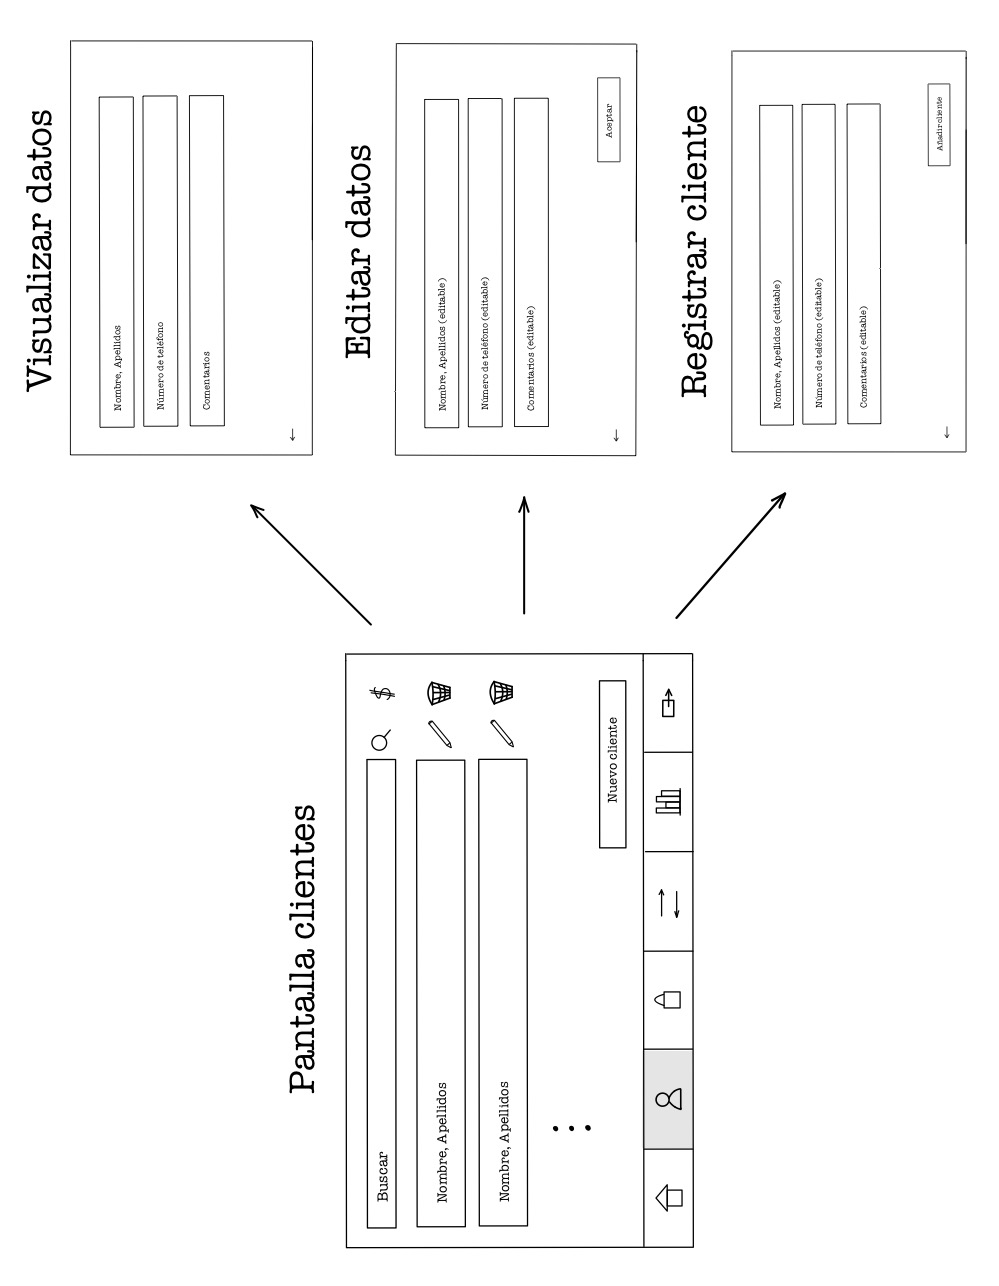
\includegraphics[width=0.8\textwidth, angle=270]{imagenes/pantalla_clientes.JPG}
	\caption{Diseño de la pantalla clientes.}
	\label{fig:pantallaclientes}
\end{figure}

\newpage

\subsection{Pantalla de artículos}

En esta sección se muestran los bocetos de la interfaz gráfica de la pantalla artículos. Estas cinco pantallas representan los requisitos RF3, RF4, RF5, RF6, RF7, RF8, RF9, RF10 y RF11. En la pantalla artículos podemos ver la lista de artículos existentes, buscar los artículos por nombre y filtrarlos por categoría. Si pulsamos encima del nombre del artículo, visualizaremos todos los datos relacionados con este. Además, podemos editar, eliminar y añadir un nuevo artículo. Por último, tenemos la lista de renovación de stock donde se introducirán todos los artículos que deba comprar el comerciante. 


\begin{figure}[ht]
	\centering
	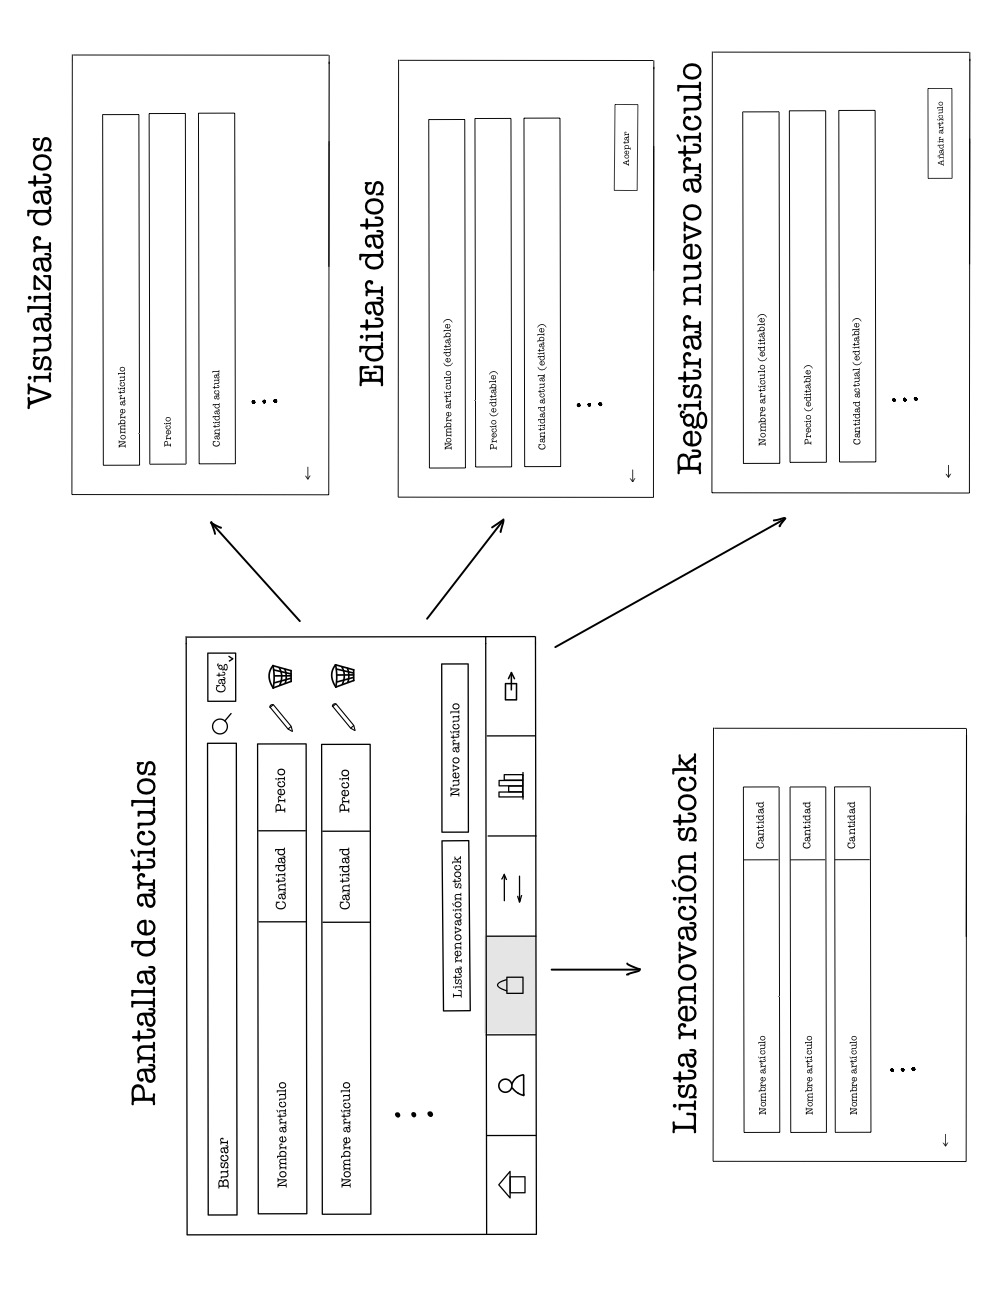
\includegraphics[width=0.8\textwidth, angle=270]{imagenes/pantalla_articulos.JPG}
	\caption{Diseño de la pantalla artículos.}
	\label{fig:pantallaarticulos}
\end{figure}

\newpage


\subsection{Pantalla de movimientos}

En esta sección se muestran los bocetos de la interfaz gráfica de la pantalla movimientos. Estas cuatro pantallas representan los requisitos RF21, RF22, RF23, RF24, RF25, RF26 y RF27. En la pantalla movimientos podemos ver la lista de movimientos existentes, buscar los movimientos por fecha o cliente asignado y filtrarlos por tipo de movimiento (venta, préstamo o devolución). Si pulsamos encima del movimiento, visualizaremos todos los datos relacionados con este. Si el movimiento es de tipo "préstamo", además de visualizarlo podremos convertirlo en venta seleccionando aquellos artículos que el cliente desea comprar. Únicamente se podrán devolver las ventas, ya que son los movimientos que generan una subida económica en la caja diaria. Las devoluciones generan una bajada correspondiente con la cantidad devuelta. Si se devuelve un préstamo sin comprar nada, se elimina el movimiento. Podemos eliminar cualquier movimiento, sea del tipo que sea. 


\begin{figure}[ht]
	\centering
	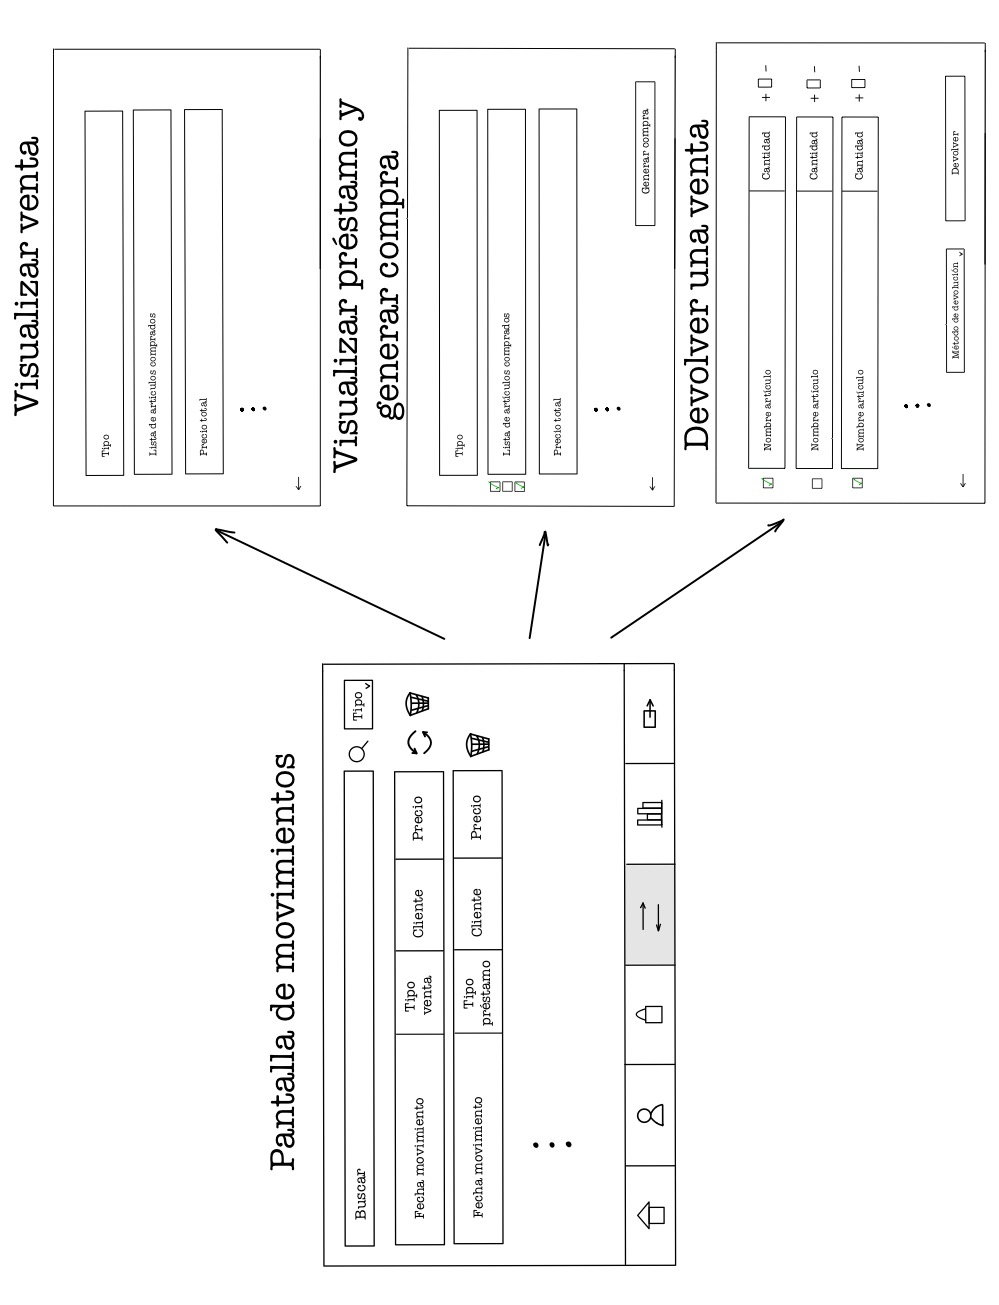
\includegraphics[width=0.8\textwidth, angle=270]{imagenes/pantalla_movimientos.JPG}
	\caption{Diseño de la pantalla movimientos.}
	\label{fig:pantallamovimientos}
\end{figure}

\newpage

\subsection{Pantalla de gráficos y cierre de sesión}

En esta sección se muestra el boceto de la interfaz gráfica de la pantalla gráficos. Esta pantalla representa el requisito RF29. Aquí podemos observar el progreso económico del negocio en forma de gráfica. Podremos verlo de forma mensual o anual. 

Para finalizar, el cierre de sesión podrá hacerse desde cualquier lugar simplemente pulsando en su botón. Esto corresponde con el requisito RF2. 


\begin{figure}[ht]
	\centering
	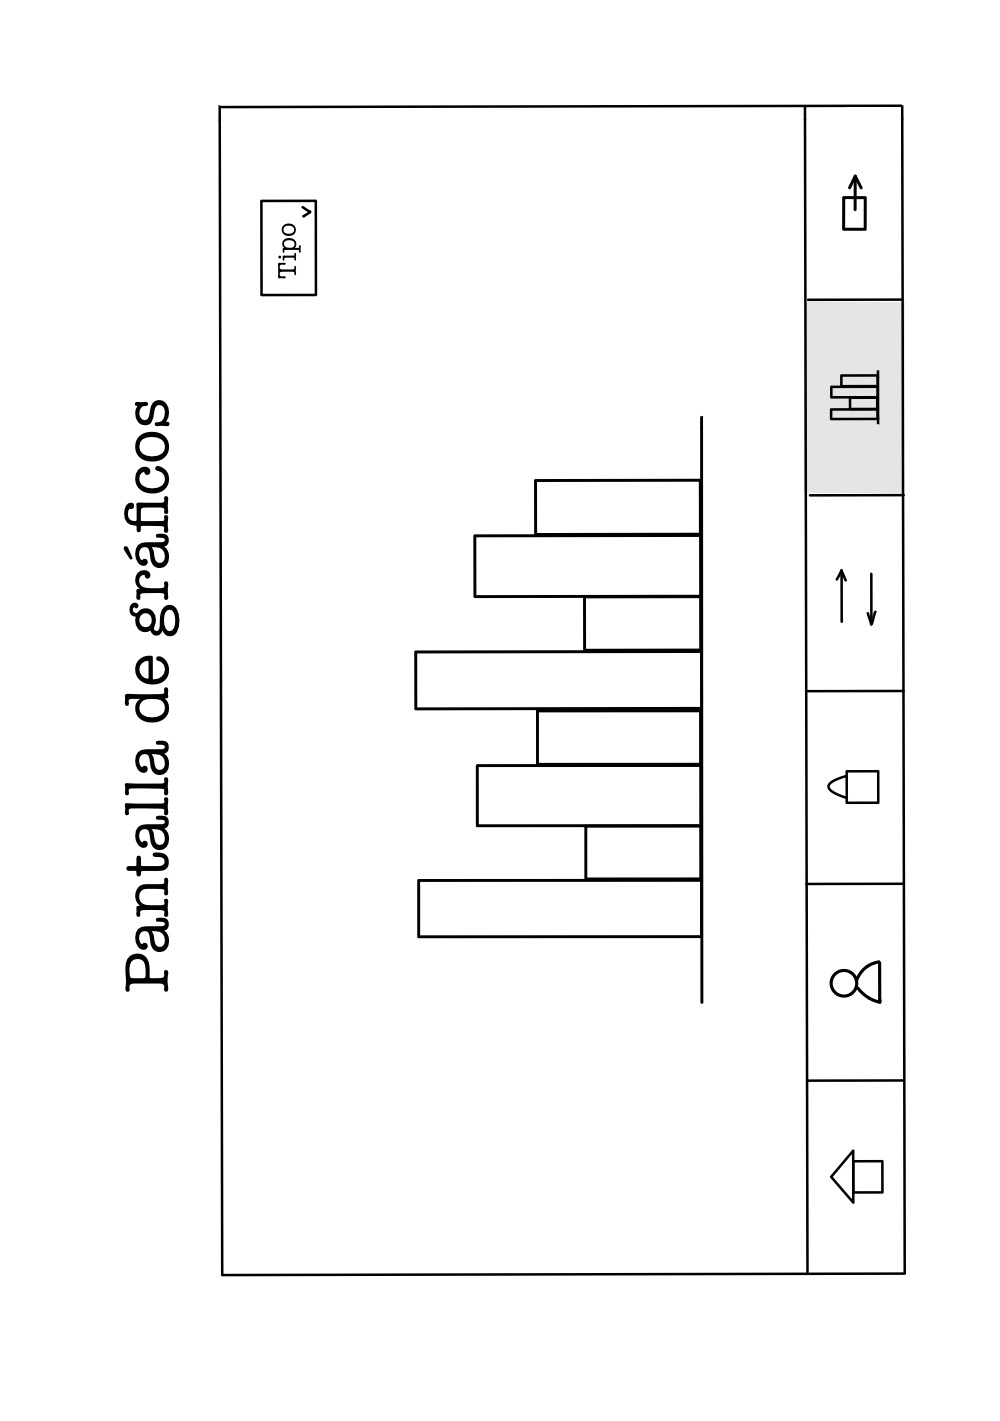
\includegraphics[width=0.8\textwidth, angle=270]{imagenes/pantalla_graficos.JPG}
	\caption{Diseño de la pantalla gráficos.}
	\label{fig:pantallagraficos}
\end{figure}